\documentclass[11pt]{book}
%\usepackage[subpreambles=true]{standalone}
\usepackage[spanish]{babel}
\usepackage{comfortaa}
\usepackage[T1]{fontenc}
\usepackage[utf8]{inputenc}
\usepackage[
letterpaper,
left=1in, 
right=1in, 
top=1in,
bottom=1in,
headheight=10mm,% Set \headheight to 10mm
]{geometry} % Custom margins
\usepackage{float}
\usepackage[colorlinks = true, linkcolor = colorrds]{hyperref}
\usepackage{bookmark}
\usepackage{fancyhdr}
\usepackage{color, colortbl}
\usepackage[dvipsnames,table]{xcolor} % Required for custom color
\usepackage{graphicx}
\usepackage{tabularx}
\usepackage{multicol,multirow}
\usepackage{newclude}
\usepackage{tabto}
\usepackage{remreset}
\usepackage[inline]{enumitem}
\usepackage{xparse}
\usepackage{wrapfig}
\usepackage{caption,capt-of}
\usepackage{amssymb,amsmath}
\usepackage{tikz}
\usepackage{etoolbox}
\usepackage{pdflscape}
\usepackage[explicit]{titlesec}
\usepackage{subfiles} % Best loaded last in the preamble
\input{insbox}
\makeatletter
\@removefromreset{section}{chapter}
\makeatother
\addto\captionsspanish{\renewcommand{\chaptername}{Unidad}}
\renewcommand{\thechapter}{\arabic{chapter}}
\renewcommand{\thesection}{S\arabic{section}}
\renewcommand{\thesubsection}{L\arabic{subsection}}
\newcommand*\chapterlabel{}
\titleformat{\chapter}
{\gdef\chapterlabel{}
    \comfortaa\Huge\bfseries
}
{\gdef\chapterlabel{\chaptername \ \thechapter}}{0pt}
{\begin{tikzpicture}[remember picture,overlay]
        \node[yshift=-2cm] at (current page.north west)
        {\begin{tikzpicture}[remember picture, overlay]
                \draw[draw=none,fill=teal] (0,0) rectangle
                (\paperwidth,2cm);
                \node[anchor=east,xshift=.9\paperwidth,rectangle,
                    rounded corners=5pt,inner xsep=20pt,inner ysep=5pt,
                    blur shadow={shadow blur steps=50,shadow blur extra rounding=5pt},
                    fill=brown]
                {\color{CadetBlue!20}\textbf{\chapterlabel#1}};
            \end{tikzpicture}
        };
    \end{tikzpicture}
}
\titlespacing*{\chapter}{0pt}{50pt}{-60pt}

\makeatletter
\@removefromreset{section}{chapter}
\makeatother
\addto\captionsspanish{\renewcommand{\chaptername}{Unidad}}
\renewcommand{\thechapter}{\arabic{chapter}}
\renewcommand{\thesection}{S\arabic{section}}
\renewcommand{\thesubsection}{L\arabic{subsection}}
\newcommand*\sectionlabel{}
\titleformat{\section}
{\gdef\sectionlabel{}
    \comfortaa\large\bfseries
}
{\gdef\sectionlabel{\thesection \ }}{0pt}
{\begin{tikzpicture}[remember picture,overlay]
        \node[yshift=-1.5cm] at (current page.north west)
        {\begin{tikzpicture}[remember picture, overlay]
                \draw[draw=none,fill=colorrds!30,
                    %shade,
                    rounded corners=5pt,
                    blur shadow={shadow blur steps=10,shadow blur extra rounding=10pt},
                    xshift=5mm,
                ] (0,0) rectangle
                (\paperwidth-10mm,2cm);
                \node[
                    anchor=west,
                    xshift=0.1\paperwidth,
                    rectangle,
                    %shade,
                    rounded corners=5pt,
                    inner sep=8pt,
                    fill=olive!50,
                    %drop shadow={fill=black, opacity=1},
                ]
                {\color{colorrds}\sectionlabel#1};
                % \node[anchor=east,xshift=.9\paperwidth,rectangle,
                %     rounded corners=10pt,inner sep=11pt,
                %     fill=blue!35]
                % {\color{green}\sectionlabel};
            \end{tikzpicture}
        };
    \end{tikzpicture}
}
\titlespacing*{\section}{0pt}{50pt}{0pt}
\usepackage[many]{tcolorbox}
% \usepackage{mathspec} 			    % for FONTS
% \usepackage{setspace}               % for LINE SPACING
% \setmainfont{Noto Sans}[
%     Kerning = On,
%     Mapping = tex-text,
%     Numbers = Uppercase,
%     BoldFont = Noto Sans SemiBold
% ]                           % setting the font as Noto Sans
% \setlength\parindent{0pt}   % killing indentation for all the text
% \setstretch{1.3}            % setting line spacing to 1.3
% \setlength\columnsep{0.25in} % setting length of column separator
% \pagestyle{empty}           % setting pagestyle to be empty


\definecolor{main}{HTML}{5989cf}    % setting main color to be used
\definecolor{sub}{HTML}{cde4ff}     % setting sub color to be used

\tcbset{
    sharp corners,
    colback = white,
    before skip = 0.2cm,    % add extra space before the box
    after skip = 0.5cm      % add extra space after the box
}                           % setting global options for tcolorbox


\newtcolorbox{bA}{
    %sharpish corners, % b
    enhanced,
    %colback = sub, % background color
    boxrule = 0.2pt,  % no borders
    %borderline = {1pt}{1pt}{black!35}, % add "dashed" for dashed line
    %fontupper = \bf\color{black}, % font color
    %colframe = main % frame color
    rounded corners,
    %arc = 5pt,   % corners roundness
    fuzzy shadow = {2pt}{-4pt}{-1pt}{1pt}{black!35}, % {xshift}{yshift}{offset}{step}{options} 
    %toprule = 3pt, % top rule weight
    %bottomrule = 3pt % bottom rule weight
}
% You can copy any following box you like to your code.
\newtcolorbox{boxA}{
    fontupper = \bf,
    boxrule = 1.5pt,
    colframe = black % frame color
}

\newtcolorbox{boxB}{
    fontupper = \bf\color{main}, % font color
    boxrule = 1.5pt,
    colframe = main,
    rounded corners,
    arc = 5pt   % corners roundness
}

\newtcolorbox{boxC}{
    colback = sub, % background color
    boxrule = 0pt  % no borders
}

\newtcolorbox{boxD}{
    colback = sub,
    colframe = main,
    boxrule = 0pt,
    toprule = 3pt, % top rule weight
    bottomrule = 3pt % bottom rule weight
}

\newtcolorbox{boxE}{
    enhanced, % for a fancier setting,
    boxrule = 0pt, % clearing the default rule
    borderline = {0.75pt}{0pt}{main}, % outer line
    borderline = {0.75pt}{2pt}{sub} % inner line
}

\newtcolorbox{boxF}{
    colback = sub,
    enhanced,
    boxrule = 1.5pt,
    colframe = white, % making the base for dash line
    borderline = {1.5pt}{0pt}{main, dashed} % add "dashed" for dashed line
}

\newtcolorbox{boxG}{
    enhanced,
    boxrule = 0pt,
    colback = sub,
    borderline west = {1pt}{0pt}{main},
    borderline west = {0.75pt}{2pt}{main},
    borderline east = {1pt}{0pt}{main},
    borderline east = {0.75pt}{2pt}{main}
}

\newtcolorbox{boxH}{
    colback = colorrds!10,
    colframe = colorrds,
    boxrule = 0pt,
    leftrule = 6pt % left rule weight
}

\newtcolorbox{boxI}{
    colback = sub,
    colframe = main,
    boxrule = 0pt,
    toprule = 6pt % top rule weight
}

\newtcolorbox{boxJ}{
    sharpish corners, % better drop shadow
    colback = sub,
    colframe = main,
    boxrule = 0pt,
    toprule = 4.5pt, % top rule weight
    enhanced,
    fuzzy shadow = {0pt}{-2pt}{-0.5pt}{0.5pt}{black!35} % {xshift}{yshift}{offset}{step}{options} 
}

\newtcolorbox{boxK}{
    sharpish corners, % better drop shadow
    boxrule = 0pt,
    toprule = 4.5pt, % top rule weight
    enhanced,
    fuzzy shadow = {0pt}{-4pt}{-1pt}{1pt}{black!35} % {xshift}{yshift}{offset}{step}{options} 
}

\newtcolorbox{boxL}{
    fontupper = \color{main},
    rounded corners,
    arc = 6pt,
    colback = sub,
    colframe = main!50,
    boxrule = 0pt,
    bottomrule = 4.5pt
}

\newtcolorbox{boxM}{
    fontupper = \color{white},
    rounded corners,
    arc = 6pt,
    colback = main!80,
    colframe = main,
    boxrule = 0pt,
    bottomrule = 4.5pt,
    enhanced,
    fuzzy shadow = {0pt}{-3pt}{-0.5pt}{0.5pt}{black!35}
}
\decimalpoint
%\captionsetup{width=.45\textwidth}
\setlength{\parindent}{0pt}
\graphicspath{{./Images}} %Setting the graphicspath
\definecolor{colorrds}{HTML}{0060A0} % Custom colour
%%% Headings and footer
\renewcommand\spanishtablename{Tabla}
\cfoot{\thepage}
\renewcommand{\headrulewidth}{0.2pt}
\renewcommand{\footrulewidth}{0.2pt}
%%%
\usetikzlibrary{
  arrows,
  positioning,
  matrix,
  calc,
  decorations.pathreplacing,
  decorations.pathmorphing,
  decorations.markings,
  decorations.text,
  shapes.symbols,
  backgrounds,
  shadows.blur,
  trees,
  fit,
  snakes,
  patterns,
  mindmap,
  intersections,
  calendar,
  plotmarks,
  spy,
  tikzmark}

%%%% APRENDISAJES TEXTBOX
\tikzset{
  abstractbox/.style={
    draw=black, fill=white, rectangle, 
    inner sep=15pt, style=rounded corners,
    drop shadow={fill=black, opacity=1}
  },
  abstracttitle/.style={fill=white}
}
\newcommand{\boxabstract}[2][fill=white]{
  \begin{tikzpicture}
    \node [abstractbox, #1] (box)
    {\begin{minipage}{0.9\linewidth}
        \setlength{\parindent}{0mm} % Indentar.
        \normalfont #2
      \end{minipage}};
    \node[abstracttitle, right=5pt] at (box.north west) {\textbf{Aprendizajes esperados:}};
    \node[draw=none, fit=(box)] {};
  \end{tikzpicture}
}%
%%%%%%%%%%%%%%%%%%%%%%%%
%\renewcommand{\labelenumi}{\mbox{\arabic{enumi}}}
%\%renewcommand{\labelitemi}{$\square$}

%%%%%%%%%%%%% START questions env
%Idea from https://tex.stackexchange.com/a/236668/1952
% \DeclareDocumentCommand\question{o}{%
%     \item\IfNoValueTF{#1}{}{(#1 puntos)}}
% \newenvironment{questions}[1][]{\enumerate[,#1]}{\endenumerate}
%\DeclareDocumentCommand\part{o}{%
% \item\IfNoValueTF{#1}{}{(#1 puntos)}}
% \newenvironment{parts}[1][]{\enumerate[,#1]}{\endenumerate}
% \newcommand{\part}{\item}
%%\newcommand{\choice}{\item}
% \newlist{parts}{enumerate*}{1}
% \setlist[parts,1]{label=(\alph*), itemjoin={{\quad}},leftmargin = 1cm}
% \newlist{oneparchoices}{enumerate*}{1}
% \setlist[oneparchoices,1]{label=\quad\alph*), itemjoin={{\quad}},leftmargin = 1cm}
% \newlist{choices}{itemize}{1}
% \setlist[choices,1]{label=\quad$\square$, itemjoin={{\\}},leftmargin = 1cm}
\newlist{hoptboxes}{itemize*}{1}
\setlist[hoptboxes,1]{label=\Large$\square$, font=\color{colorrds},itemjoin={{\quad}},leftmargin = 1cm}
\newlist{hoptions}{enumerate*}{1}
\setlist[hoptions,1]{label=(\alph*), font=\color{colorrds},itemjoin={{\quad}},leftmargin = 1cm}
%%%%%%%%%%%%% END questions env
\newenvironment{mybox}[3][]{%
  \begin{tikzpicture}[#1]%
    \def\myboxname{#3}%
    % good options: minimum height, minimum width
    \node [draw, inner sep=2ex,  align=justify]
      (BOXCONTENT) \bgroup\rule{0ex}{0ex}\ignorespaces
  }{%
    \egroup;
    \node [right, inner sep=3pt, fill=colorrds!75, outer sep=0pt, 
      text height=2ex, text depth=.5ex] (BOXNAME) 
      at ([shift={(-1em,5pt)}]BOXCONTENT.north west) {\myboxname};
    \fill[colorrds] (BOXNAME.north east) -- +(-1em,1em)
      -- +(-1em,0) -- cycle;
    \fill[colorrds] (BOXNAME.south west) -- +(1em,-1em)
      -- +(1em,0) -- cycle;
  \end{tikzpicture}
}
\begin{document}
\pagestyle{empty}
\newgeometry{left=0mm,top=50mm,bottom=0mm,right=0mm}
\documentclass[]{book}
\usepackage{geometry,graphicx} % Custom margins
\usepackage[spanish]{babel}
\usepackage[T1]{fontenc}
\usepackage[dvipsnames]{xcolor} % Required for custom color
\usepackage{color,colortbl}
\usepackage[utf8]{inputenc}
\usepackage{geometry} % Custom margins
\usepackage[spanish]{babel}
\usepackage{adjustbox,dashbox}
\usepackage{array}
\usepackage{tikz,pgfplots,pgfkeys}
\usepackage{forest,mathtools,siunitx}
\usepackage{amsfonts, amssymb, amsxtra, amsmath, amsbsy}
\usepackage{newclude}
\usepackage{ifthen}
\usepackage{float}
\usepackage{fancybox}
\usepackage{graphicx,tabularx}
\usepackage{multicol,multirow}
\usepackage{enumitem} % Customising the numbered lists
\usepackage{xhfill} % Making the pink block not extend beyond the margin
\usepackage{nameref} % reference the names of the sections
\usepackage{caption,capt-of}
\usepackage[normalem]{ulem} % Dashed lines in appendix
\usepackage{ragged2e} % Ragged left
\usepackage{booktabs}
\usepackage[unboxed]{cwpuzzle}
\usepackage[colorlinks = true,linkcolor = blue]{hyperref}
\usepackage{subfiles}
\usepackage{wrapfig}
\input{insbox}
\usepackage{etoolbox}
\usepackage{mwe}
\usepackage{comfortaa}
\usepackage[T1]{fontenc}
\renewcommand*\oldstylenums[1]{{\firaoldstyle #1}}
\usepackage[T1]{fontenc}
\usepackage{pythontex}
\usepackage{polynom}
\usepackage{longdivision}


\title{Actividades}
\author{Julio C. Melchor P.\thanks{{\tt julio.melchor@rafaeldiazserdan.net}}}
\date{v1.0, \today}
%\usepackage[dvipsnames]{xcolor} % Required for custom color
\usepackage{color,colortbl}
\usepackage[utf8]{inputenc}
\usepackage{geometry} % Custom margins
\usepackage[spanish]{babel}
\usepackage{adjustbox,dashbox}
\usepackage{array}
\usepackage{tikz,pgfplots,pgfkeys}
\usepackage{forest,mathtools,siunitx}
\usepackage{amsfonts, amssymb, amsxtra, amsmath, amsbsy}
\usepackage{newclude}
\usepackage{ifthen}
\usepackage{float}
\usepackage{fancybox}
\usepackage{graphicx,tabularx}
\usepackage{multicol,multirow}
\usepackage{enumitem} % Customising the numbered lists
\usepackage{xhfill} % Making the pink block not extend beyond the margin
\usepackage{nameref} % reference the names of the sections
\usepackage{caption,capt-of}
\usepackage[normalem]{ulem} % Dashed lines in appendix
\usepackage{ragged2e} % Ragged left
\usepackage{booktabs}
\usepackage[unboxed]{cwpuzzle}
\usepackage[colorlinks = true,linkcolor = blue]{hyperref}
\usepackage{subfiles}
\usepackage{wrapfig}
\input{insbox}
\usepackage{etoolbox}
\usepackage{mwe}
\usepackage{comfortaa}
\usepackage[T1]{fontenc}
\renewcommand*\oldstylenums[1]{{\firaoldstyle #1}}
\usepackage[T1]{fontenc}
\usepackage{pythontex}
\usepackage{polynom}
\usepackage{longdivision}

 % Imports all the required packages. See Functional/%Packages.tex for more detailS
\geometry{letterpaper,total={175mm,220mm},left=15mm,top=50mm,bottom=0mm} % Custom margins

\begin{document}
\pagestyle{empty}
\begin{center}
    {\Huge Matem\'aticas 3}\\
    \vspace{1cm}
    \normalsize
    \textbf{\large Cuaderno de trabajo}\\
    para los alumnos de 3$^\circ$ de  Secundaria\\
    en el curso durante el ciclo escolar\\
    \textbf{2022-2023}\\
    \vspace{2.2cm}
    \small POR\\
    \Large J. C. Melchor Pinto\\[0.5em]
    \normalsize Profesor de asignatura en\\
    \vspace{1cm}
    
\includegraphics[width=5cm]{../Unidad 2/Images/LOGO_RDS_nobg}
\end{center}
\vspace{2.5cm}
%\include*{Functional/TitlePage}
\hspace{-16mm}
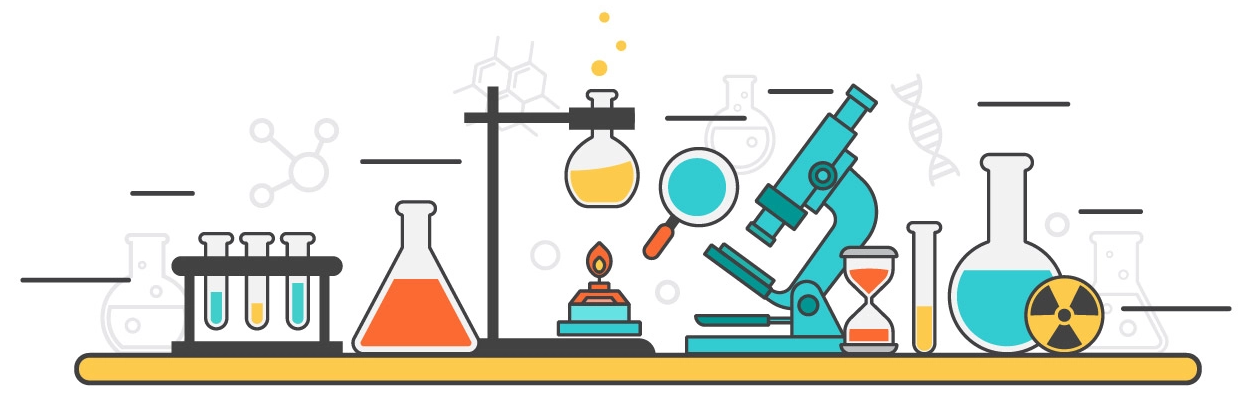
\includegraphics[width=\paperwidth]{../Unidad 2/Images/cover_bg}
\end{document}

\restoregeometry
\addtocontents{toc}{\setcounter{tocdepth}{3}}
\tableofcontents
\newpage
\chapter{}
\pagestyle{fancy}
\newpage
\newpage \thispagestyle{plain}
\section{Nuestro mundo químico}
\subsection{La química en tu vida y el medio ambiente }

\newpage \thispagestyle{plain}
\section{Los materiales, las sustancias\\ y sus propiedades}
This is a sample of a section
\subsection{¿Cómo sabemos que un material es distinto de otro?}
\subsection{¿Cómo podemos medir las propiedades de los materiales?}
\newpage \thispagestyle{plain}
\section{Relación entre propiedades de las sustancias e intercambios de energía}
\subsection{¿Cómo utilizamos energía para analizar sustancias?}

\newpage \thispagestyle{plain}
\section{Mezclas: propiedades y métodos de separación}

\subsection{Propiedades y clasificación de las mezclas}

\newpage \thispagestyle{plain}
\section{Mezclas y sustancias contaminantes}
\subsection{¿Cómo detectamos y prevenimos la presencia de sustancias nocivas en el medio ambiente?}

\subsection{Métodos de separación de mezclas}

\newpage \thispagestyle{plain}
\section{Sustancias elementales y sus propiedades}
\subsection{¿Hay sustancias más simples que otras?}
\subsection{Regularidades en las propiedades\\ de las sustancias elementales}

\newpage
\chapter{}
% \begin{minipage}{.45\textwidth}
%   \begin{figure}[H]
%     \centering
%     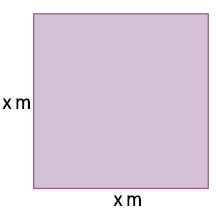
\includegraphics[width=0.7\linewidth]{square.png}
%     \captionof{figure}{Modelo geométrico de la situación.}
%     \label{fig:square}
%   \end{figure}%
% \end{minipage}\hfill
% \begin{minipage}{.45\textwidth}
%   \begin{figure}[H]
%     \centering
%     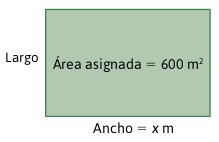
\includegraphics[width=0.8\linewidth]{square2.png}
%     \captionof{figure}{Modelo geométrico de la situación.}
%     \label{fig:square2}
%   \end{figure}
% \end{minipage}
\newpage \thispagestyle{plain}
\section{La estructura de la materia y sus modelos}
\boxabstract{
  \begin{itemize}
    \item Deduce información acerca de la estructura atómica
          a partir de datos experimentales sobre propiedades
          atómicas periódicas.
    \item Representa y diferencia mediante esquemas, modelos y
          simbología química, elementos y compuestos, así como
          átomos y moléculas.
    \item Explica y predice propiedades físicas de los materiales
          con base en modelos submicroscópicos sobre la
          estructura de átomos, moléculas o iones, y sus
          interacciones electrostáticas.
  \end{itemize}
}
\newpage
\subsection{¿Cómo los átomos y las moléculas hacen distintas a las sustancias?}

\begin{boxK}
  \begin{enumerate}
    \item Anota en la tabla dos propiedades que distinguen a las sustancias que se indican y con
          las que de seguro estás en contacto frecuentemente.
    \item Dibuja qué verías si observaras cada sustancia con un microscopio muy potente.
    \item Compara tus ideas y dibujos con los de un compañero y comenten: \\
          \textbf{¿cómo explican sus dibujos las propiedades macroscópicas de las sustancias que representaron?}
          \begin{figure}[H]
            \centering
            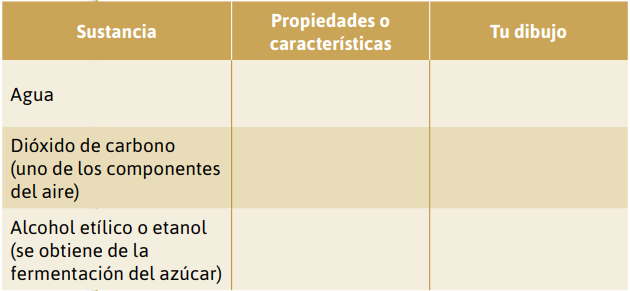
\includegraphics[width=0.7\linewidth]{tabla01.png}
            %\captionof{table}{Modelo geométrico de la situación.}
            \label{tab:tabla01}
          \end{figure}%
  \end{enumerate}
\end{boxK}

\subsubsection{Átomos y moléculas}

¿Por qué el carbón es una sustancia sólida negra y quebradiza que se quema con facilidad?
¿Por qué el azúcar es dulce y se disuelve en el agua? A lo largo de la historia, los químicos han realizado
diversos experimentos para comprender por qué cada sustancia tiene propiedades distintas.
\begin{wrapfigure}{l}{0.48\textwidth}
  \centering
  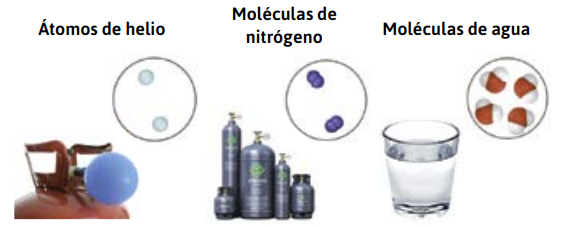
\includegraphics[width=\linewidth]{atomos01.png}
  \captionof{figure}{\footnotesize Representación de las partículas que constituyen diversas
    sustancias. Los átomos de distintos tipos se representan comúnmente
    como esferas de diferente color.}
  \label{fig:atomos01}
\end{wrapfigure}
Los resultados experimentales se pueden explicar mediante el modelo
cinético de partículas que estudiaste en tu curso de Ciencia y tecnología, Física, el cual supone que:


%\begin{boxM}
\begin{itemize}
  \item[\checkmark] Las sustancias están constituidas por miles de millones de partículas pequeñísimas
        en constante movimiento e interacción;
  \item[\checkmark] Las partículas de una sustancia son idénticas entre sí y tienen una composición y
        estructura determinadas, que son diferentes a las de otras sustancias;
  \item[\checkmark] Las partículas de cada sustancia por lo general están constituidas por unidades más
        pequeñas llamadas \textbf{átomos}, unidos unos a otros por fuerzas de atracción llamadas \textbf{enlaces químicos}.
\end{itemize}
%\end{boxM}

Algunas sustancias elementales, como el helio y el argón, están constituidas por partículas de un solo átomo; sin embargo, las
partículas de muchas otras sustancias se forman por la unión, mediante enlaces químicos, de dos o más átomos; a estas partículas
se les llama \textbf{moléculas} (figura \ref{fig:atomos01}).

Por ejemplo, el gas nitrógeno del aire está constituido por moléculas de dos átomos
idénticos, mientras que las moléculas de agua están formadas por dos átomos de
hidrógeno unidos a un átomo de oxígeno (átomos de diferente tipo).
Las diferencias en las propiedades de las sustancias se deben a los distintos tipos
y números de átomos de las partículas que las constituyen y a la forma en que los
átomos se enlazan unos a otros.\\

\begin{boxK}
  \begin{wrapfigure}{r}{0.25\textwidth}
    \centering
    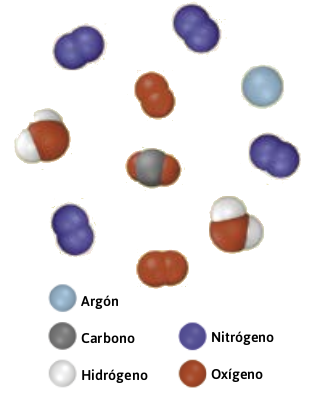
\includegraphics[width=0.25\textwidth]{atomos02.png}
    \label{fig:atomos02}
  \end{wrapfigure}
  Analiza y reflexiona:\\
  \begin{enumerate}
    \item Observa la representación de las partículas que
          forman algunas sustancias del aire que respiras.
          El código de color que por lo común se utiliza
          para representar átomos de distintos tipos es el
          que se muestra.
    \item Determina cuántas sustancias distintas se representan.
    \item Determina qué sustancias están constituidas por átomos independientes y cuáles por moléculas.
    \item Describe las semejanzas y diferencias de las moléculas que identificaste: considera tipo y cantidad de átomos.
    \item Compara tus respuestas con las de tus compañeros y valídenlas.
  \end{enumerate}%
  % \end{minipage}
\end{boxK}

\subsubsection{Sustancias elementales y compuestos químicos a nivel nanoscópico}

Como estudiaste en la unidad anterior, existen sustancias elementales que no se pueden descomponer
en otras más simples mediante procesos químicos. El nitrógeno y el oxígeno del aire son
ejemplos de sustancias elementales. Por otro lado, los compuestos
químicos sí se descomponen en sustancias elementales a partir
de métodos químicos. Algunos ejemplos son el agua, que puede
descomponerse en hidrógeno y oxígeno, y el dióxido de carbono
que exhalamos, que se descompone en oxígeno y carbono.\\

\begin{wrapfigure}{r}{0.3\textwidth}
  \centering
  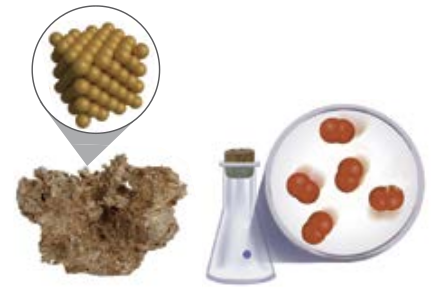
\includegraphics[width=0.3\textwidth]{atomos03.png}
  \captionof{figure}{\footnotesize El cobre y el oxígeno son sustancias
    elementales constituidas por átomos del mismo
    tipo.}
  \label{fig:atomos03}
\end{wrapfigure}

La idea de que las sustancias están constituidas por diferentes
tipos de átomos permite explicar la diferencia entre sustancias elementales y
compuestos químicos. Las elementales no pueden descomponerse en sustancias más simples porque están constituidas
por partículas con el mismo tipo de átomo.\\

\begin{wrapfigure}{l}{0.3\textwidth}
  \centering
  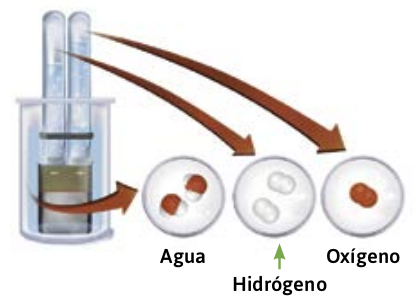
\includegraphics[width=0.3\textwidth]{atomos04.png}
  \captionof{figure}{\footnotesize El agua se logra descomponer en
    hidrógeno y oxígeno mediante el paso de
    corriente eléctrica.}
  \label{fig:atomos04}
\end{wrapfigure}

Por ejemplo, el cobre
con el que se fabrican cables, está conformado por átomos idénticos ordenados uno junto a otro,
mientras que el oxígeno que respiramos tiene moléculas con dos átomos de oxígeno cada una (figura
\ref{fig:atomos03}). Por su parte, los compuestos químicos se pueden descomponer en sustancias elementales porque están constituidos por partículas
con átomos de distintos tipos. Los átomos que conforman las moléculas de agua, por ejemplo, se pueden separar y reorganizarse para
formar las sustancias elementales hidrógeno y oxígeno (figura \ref{fig:atomos04}).\\

\subsubsection{Tipos de \'atomos}

La separación e identificación de las diferentes sustancias elementales que
hay en la naturaleza ha permitido determinar los distintos tipos de átomos
que existen. En la actualidad se han identificado más de 100 átomos
distintos, y las partículas de todas las sustancias conocidas, natu-
rales o sintéticas, son resultado de la combinación de esos átomos
(figura 2.4). Cada tipo de átomo corresponde con un elemento
químico y se le asigna un símbolo particular.

Por ejemplo, los
átomos de oxígeno se representan con el símbolo \emph{O}, mientras que
los átomos de hidrógeno, con el símbolo \emph{H}. Los símbolos que repre-
sentan cada tipo de átomo no siempre corresponden con las primeras letras
de su nombre en español, porque algunos se derivan del nombre de las sus-
tancias en otros idiomas, como el latín.\\

\begin{minipage}{\textwidth}
  \begin{boxK}
    Observa y representa:

    \begin{enumerate}
      \item Distingue similitudes y diferencias en las representaciones de las siguientes
            moléculas de distintas sustancias.

            \begin{figure}[H]
              \centering
              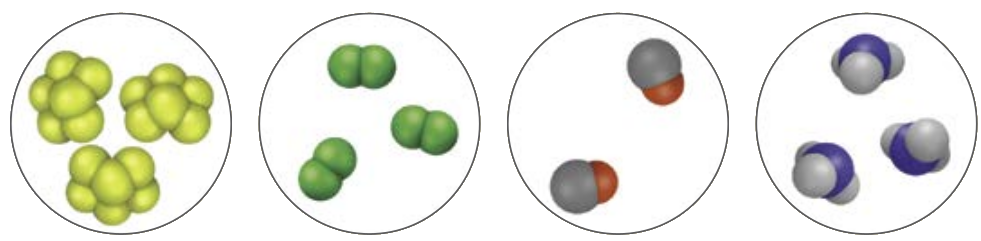
\includegraphics[width=.6\textwidth]{atomos05.png}
            \end{figure}

      \item Identifica cuáles representan sustancias elementales y cuáles compuestos quí-
            micos. Justifica tus decisiones.
      \item Usa las representaciones anteriores para representar una mezcla constituida por
            partículas de una sustancia elemental y partículas de un compuesto químico.
      \item Compara y contrasta tus dibujos con los de tus compañeros.
    \end{enumerate}
  \end{boxK}
\end{minipage}
\vspace{0.5cm}

\begin{wrapfigure}{l}{0.4\textwidth}
  \centering
  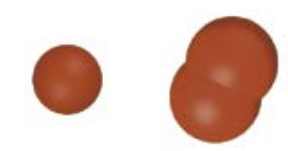
\includegraphics[width=0.3\textwidth]{atomos07.png}
  \captionof{figure}{\footnotesize Las propiedades y estructura de estas sustancias son diferentes aunque tengan el mismo tipo de átomo.}
  \label{fig:atomos07}
\end{wrapfigure}

Para el sodio, por ejemplo, el símbolo es Na porque proviene de su nombre en latín, natrium, que significa raro.
Los diferentes átomos o elementos químicos conocidos se listan en la
tabla periódica de los elementos (figura 2.6, p. 103). Los que se localizan en la misma hilera pertene-
cen al mismo periodo. Los átomos o elementos incluidos en la tabla periódica tienen el mismo
nombre que la sustancia elemental en la que están presentes, pero las pro-
piedades de esos átomos no son las mismas que las de las sustancias ele-
mentales.\\

\begin{wrapfigure}{l}{0.45\textwidth}
  \centering
  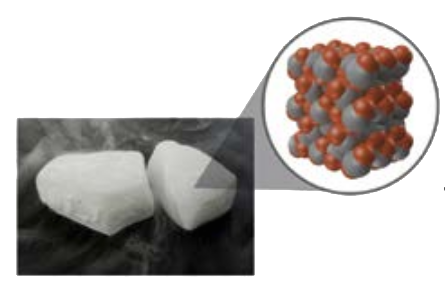
\includegraphics[width=0.45\textwidth]{atomos06.png}
  \captionof{figure}{\footnotesize El hielo seco (dióxido de
    carbono sólido) es un compuesto químico constituido por los elementos carbono y oxígeno.}
  \label{fig:atomos06}
\end{wrapfigure}

Por ejemplo, el oxígeno gaseoso presente en el aire que respiramos
está constituido por moléculas de dos átomos de oxígeno cada una. Los seres
humanos inhalamos sin problema las moléculas de oxígeno contenidas en
el aire, pero si en lugar de moléculas respiráramos átomos de oxígeno sepa-
rados, podríamos morir (figura 2.5).\\

Las propiedades de las sustancias elementales no sólo de-
penden del tipo de átomos que las componen, sino también
de cómo estos se enlazan en las partículas que los constitu-
yen. Por ejemplo, el grafito que contiene la punta de los lápi-
ces es una sustancia elemental suave y quebradiza hecha de
átomos de carbono (C), mientras que el diamante, que es duro
y resistente, también es una sustancia elemental formada por
átomos de carbono (figura 2.7).\\

\begin{boxK}
  Analiza y genera hipótesis
  \begin{enumerate}
    \item Discute con tus compañeros sobre cómo es posible que
          dos sustancias con propiedades tan distintas como el
          diamante y el grafito estén constituidas por el mismo
          tipo de átomos (carbono, C).
  \end{enumerate}
\end{boxK}

\subsubsection{Simbología química}

Los químicos han desarrollado distintas maneras de representar la composición y
estructura de las sustancias elementales y de los compuestos químicos de nuestro
entorno (nivel macroscópico) mediante dibujos que representan los átomos y moléculas presentes en el material. Cuando describimos el comportamiento de las sustancias
y los materiales representando los átomos y moléculas que los forman se dice que
hacemos una descripción a nivel nanoscópico.
En estas representaciones usamos fórmulas químicas que se hacen a partir de los
símbolos de los átomos o elementos químicos. Si las moléculas poseen átomos iguales,
se usan subíndices para indicar el número de átomos de cada tipo. Por ejemplo, la
fórmula química de las moléculas del oxígeno que respiramos es O$_2$ , lo cual indica que
cada una está constituida por dos átomos de oxígeno. La fórmula química de las moléculas de dióxido de carbono es CO$_2$ ; esto indica que están formadas por un átomo de
carbono y dos de oxígeno. Si se necesita representar una sustancia con gran cantidad
de partículas en estado sólido, líquido o gaseoso, los símbolos (s), (l) y (g) se colocan a
la derecha de la fórmula: CO$_2$ (s) representa una muestra de dióxido de carbono sólido
(hielo seco) y O$_2$ (g) representa una muestra de oxígeno gaseoso.

En esta lección has aprendido que las diferencias en las propiedades de las sustancias
se deben a la composición de las partículas que las constituyen, la cual se representa
mediante esquemas que muestran la composición atómica de las partículas o el uso
de fórmulas químicas. Para evaluar lo que has aprendido, haz la siguiente actividad.

\newpage
\begin{boxK}
  \begin{enumerate}
    \item Completa la información de la tabla.
    \item Compara y contrasta la composición de las partículas que constituyen las distintas sustancias.
    \item Compara estas representaciones con las que hiciste al inicio de esta lección
          (p. 100): ¿cómo cambiaron? ¿Qué ventajas y desventajas tiene una representación respecto a la otra?
          \begin{figure}[H]
            \centering
            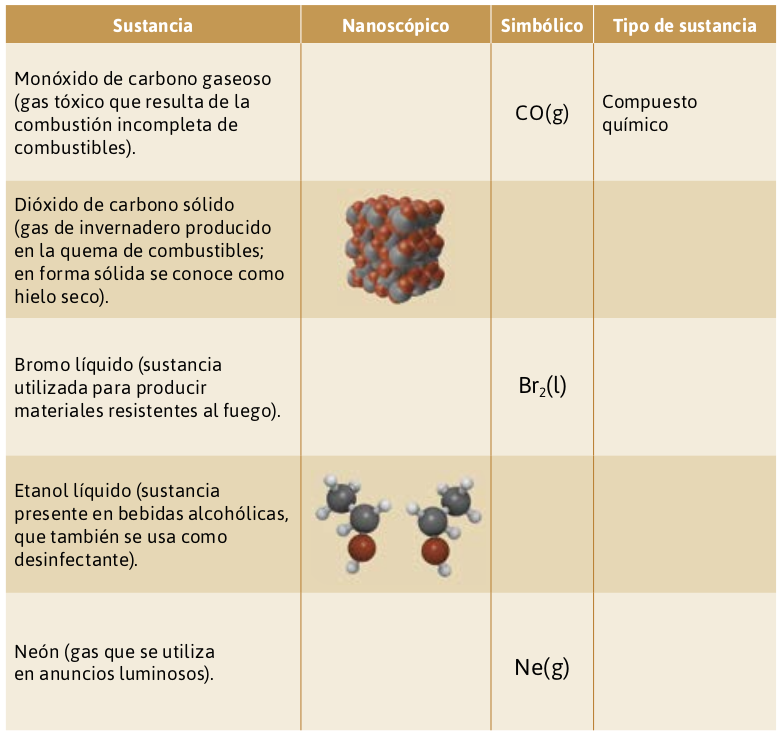
\includegraphics[width=.8\textwidth]{tabla02.png}
          \end{figure}

  \end{enumerate}
\end{boxK}

\newpage
\subsection{¿Qué hace a un átomo diferente de otro?}

\begin{boxK}
  \begin{enumerate}
    \item Explora las propiedades eléctricas de distintos materiales; por ejemplo, infla un globo
          (también puedes utilizar un vaso de plástico) y frótalo sobre tu cabello. Enseguida,
          acerca el globo a distintos materiales, como pequeños trozos de papel,
          una bolsa de plástico, un vaso de unicel, una lata de aluminio o un
          chorro fino de agua y de otras sustancias.
    \item Observa qué pasa en cada caso.
    \item Discute con tus compañeros por qué piensas que el material del que
          está hecho el globo interacciona de diferentes maneras con los otros
          materiales. Recuerda lo que aprendiste en tu curso de Ciencia y tec-
          nología, Física sobre interacciones eléctricas.
    \item Discutan qué sucede a nivel nanoscópico con los átomos y las molécu-
          las de las que están hechos estos materiales cuando los frotan.
  \end{enumerate}

\end{boxK}

\subsubsection{Componentes atómicos}

Un gran número de experimentos, como el propuesto en la actividad de inicio, sugie-
ren que la materia tiene propiedades eléctricas. En tu curso de Física aprendiste que
científicos como Thomson y Rutherford, a partir de distintos experimentos, detectaron
partículas (llamadas subatómicas) con cargas positivas y negativas en los átomos
y moléculas que constituyen las sustancias químicas. Con esta información propusie-
ron modelos para describir la estructura de los átomos, como el que se representa en
la figura 2.8.\\

\begin{figure}[H]
  \centering
  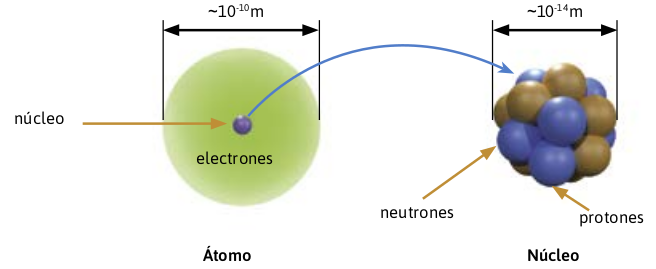
\includegraphics[width=0.7\linewidth]{atomos08.png}
  %\captionof{table}{Modelo geométrico de la situación.}
  \label{tab:atomos08}
\end{figure}%

De acuerdo con este modelo atómico, cada átomo está constituido por partículas
con carga positiva, llamadas protones, concentradas en un núcleo muy pequeño, y por
partículas con carga negativa, denominadas electrones, que se mueven a su alrededor.
El núcleo de los átomos contiene otro tipo de partículas sin carga eléctrica (partículas
neutras) conocidas como neutrones. Los electrones son partículas muy pequeñas y
ligeras (poca masa), mientras que los protones y neutrones son de mayor tamaño y
poseen una masa 2 000 veces mayor que la del electrón. Cada átomo tiene el mismo
número de protones que de electrones y, por tanto, es eléctricamente neutro. Los elec-
trones se mantienen en movimiento alrededor del núcleo por la atracción entre cargas
eléctricas negativas y positivas.


\begin{boxK}
  Compara y analiza:\\
  \begin{enumerate}
    \item Lee y usa la información que se muestra en la imagen para determinar cuántas
          veces es más pequeño un átomo comparado con los objetos y organismos. Si es
          necesario, investiga el valor de las unidades de medida representadas.

          \begin{figure}[H]
            \centering
            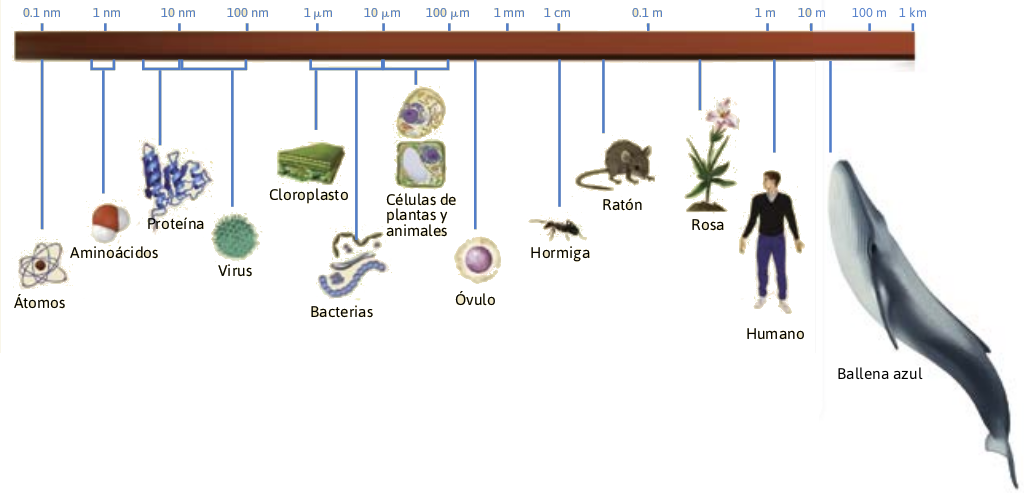
\includegraphics[width=.9\textwidth]{escala.png}
          \end{figure}

          Los átomos son partículas muy pequeñas. En el diámetro de uno de tus cabellos se podrían
          acomodar en hilera unos 500 000 átomos de carbono. Si un cabello se pudiera agrandar
          hasta alcanzar el diámetro de nuestro planeta, un átomo del cabello tendría el tamaño de
          una cancha de basquetbol.

    \item Compara tus respuestas y métodos con los de otros compañeros y valídenlos.
  \end{enumerate}
\end{boxK}
\newpage
\subsection{¿Cómo estudiamos a los átomos de manera experimental?}

\newpage \thispagestyle{plain}
\section{Composición y estructura de distintos tipos de sustancias}

\boxabstract{
  \begin{itemize}
    \item Representa y diferencia mediante esquemas, modelos y
          simbología química, elementos y compuestos, así como
          átomos y moléculas.
    \item Explica y predice propiedades físicas de los materiales
          con base en modelos submicroscópicos sobre la
          estructura de átomos, moléculas o iones, y sus
          interacciones electrostáticas.
  \end{itemize}
}
\subsection{¿Qué tipos de partículas se forman al combinar los átomos?}

\newpage \thispagestyle{plain}
\section{Moléculas de importancia para la vida}
\boxabstract{
  \begin{itemize}
    \item Identifica componentes químicos importantes
          (carbohidratos, lípidos, proteínas, ADN) que participan en
          la estructura y funciones del cuerpo humano.
    \item Representa y diferencia mediante esquemas, modelos y
          simbología química, elementos y compuestos, así como
          átomos y moléculas.
    \item Explica y predice propiedades físicas de los materiales
          con base en modelos submicroscópicos sobre la
          estructura de átomos, moléculas o iones, y sus
          interacciones electrostáticas.
  \end{itemize}
}
\subsection{¿Qué moléculas nos constituyen?}

\newpage \thispagestyle{plain}
\section{Relaciones entre la estructura y las propiedades de las sustancias}
\boxabstract{
  \begin{itemize}
    \item Representa y diferencia mediante esquemas, modelos y
          simbología química, elementos y compuestos, así como
          átomos y moléculas.
    \item Explica y predice propiedades físicas de los materiales
          con base en modelos submicroscópicos sobre la
          estructura de átomos, moléculas o iones, y sus
          interacciones electrostáticas.
  \end{itemize}
}
\subsection{¿Cómo interaccionan las moléculas?}
\subsection{¿Cómo se explican y predicen las propiedades de las sustancias?}

\newpage \thispagestyle{plain}
\section{Reacciones químicas en nuestro mundo}
\subsection{¿Cuál es la evidencia de que las sustancias reaccionan unas con otras?}

\newpage \thispagestyle{plain}
\section{Recombinaciones atómicas}
\subsection{¿Cómo representamos las reacciones químicas?}
\subsection{¿Qué cambia y qué se conserva durante las reacciones químicas?}

\newpage \thispagestyle{plain}
\section{Cantidad de las sustancias}
\subsection{¿Cómo determinamos la cantidad de las sustancias?}
\subsection{Cantidad de las sustancias en reacciones químicas}

\newpage
\chapter{}

\newpage \thispagestyle{plain}
\section{Un mundo de reacciones químicas}
\subsection{¿Cómo nos afectan las reacciones químicas?}
\subsection{¿Cómo aprovechamos las reacciones químicas?}

\newpage \thispagestyle{plain}
\section{Energía y reacción química}
\subsection{¿Cómo se transfiere energía durante las reacciones químicas?}
\subsection{¿Por qué se transfiere energía durante las reacciones químicas?}

\newpage \thispagestyle{plain}
\section{La energía química en nuestras vidas}
\subsection{¿Cuáles son los beneficios, costos y riesgos de usar energía química?}

\newpage \thispagestyle{plain}
\section{Aporte calórico de los alimentos}
\subsection{¿De dónde proviene la energía que necesitamos para vivir?}

\newpage \thispagestyle{plain}
\section{Rapidez de reacción}
\subsection{¿Qué factores afectan la rapidez de las reacciones químicas?}

\newpage \thispagestyle{plain}
\section{La rapidez de reacción y el modelo cinético de partículas}
\subsection{¿Cómo explicamos diferencias en la velocidad de reacción?}

\newpage \thispagestyle{plain}
\section{Utilidad de controlar la rapidez de las reacciones}
\subsection{¿Cómo controlamos y aprovechamos la velocidad de reacción?}

\end{document}